\chapter{Text-Guided Image Editing}
\label{chapter:flexit}

\newpage

\minitoc
\chapterwithfigures{\nameref*{chapter:flexit}}
\chapterwithtables{\nameref*{chapter:flexit}}

\ifthenelse{\boolean{skipFlexit}}{\endinput}{}

\todo{in pres: in practice: how well are the text and image pairs aligned? can i perform vector arithmetic? let's see what it does?}
\todo{talk about IC-GAN}

\section{Introduction}

Thusfar, we have examined one way of performing semantic-image editing: 
generalizing latent manipulation methods of \ac{GAN}s to real images. For this, 
we saw in the previous chapter that the real image must first be inverted into 
the latent space of a \ac{GAN}, a task that is not trivial and will poorly respond to 
 images out of the \ac{GAN}'s distribution. Moreover, we saw that in general, \ac{GAN}s 
 are highly powerful in generating images of a restricted domain, they are much less 
 efficient in generating high-quality and diverse images of a more diverse domain. 
 However, we strive to perform image editing on any possible image. In this chapter, 
 we thus investigate the use of a recently proposed autoencoder, VQ-GAN \citep{esser2021taming}, 
 to bypass this issue and encode any image into a latent "code" directly. 
 
Specifically, we propose  a unified framework which modifies an input image based
 on a user-defined text query of the form $(S \rightarrow T)$, like \textit{cat} → \textit{dog}.
  For this \textit{semantic image translation} task, the goal is to make minimal image
   modifications  while transforming the image as requested.
We leverage \ac{CLIP} \citep{radford2021learning},  which combines text and image representations in 
one powerful multimodal embedding space. This space is used to define our target point,
 based on the embeddings from the user input. We perform a per-image optimization 
 procedure, using specific  strategies to ensure image quality and relevance to the 
 transformation query. Our method requires only fixed pre-trained components, and can 
 thus be used off-the-shelf  without  requiring any training. 

We also propose a quantitative evaluation protocol for the task of semantic image 
translation. 
Evaluation is based on three criteria: (i) the transformed image should correctly 
correspond to the text query, (ii) the output image should look natural,  and (iii) 
visual elements irrelevant to the text query should remain unchanged. 
We thoroughly evaluate our model on ImageNet, and  demonstrate quantitatively and 
qualitatively the superiority of our method against baselines, broadening the horizon 
of text-driven image editing.


\section{Related Work}

% talk about Instance GAN

% takl about manigan


\paragraph{Image latent space}
While GANs are highly effective as generative models, inference of the latent variable 
given an image is not trivial, as we have seen in Chapter \ref{chapter:magec}. 
While joint learning of an inference network has been proposed, \citep{donahue17iclr,dumoulin17iclr}, 
the mode-seeking training dynamics of GANs are 
 not suited for good reconstruction performance beyond the training distribution 
 (or even within it, if modes are dropped).
Variational autoencoders~\cite{Kingma2014}, on the other hand, offer an inference 
network by construction, and their likelihood-based training objective ensures accurate 
reconstructions.

Vector-quantized  variational autoencoders (VQ-VAE)~\cite{oord17nips,razavi2019generating},
 which discretize the latent space, have been found to offer good reconstructions. The prior distribution
 is a categorical distribution and kept constant and uniform during sampling.
 The prior is not trained jointly with with VQ-VAE, and thus, unlike classical \ac{VAE}s (see \ref{section:chapter1_variational_auto_encoders}),
 has no generative capacities until it is made autoregressive (which is done in a next step). 
VQ-GAN \citep{esser2021taming,yu2021vector} further improves reconstructions 
by  including an adversarial loss term to train the autoencoder.
In our work,  we adopt the VQ-GAN autoencoder,  and edit  images in its latent space.



\paragraph{CLIP and Text-Guided image editing}

To align images and text, \ac{CLIP}~\citep{radford2021learning} learns encoders that map both 
modalities to a shared latent space in which they can easily be compared and combined.
 Vision encoders are based on ResNets \citep{he2016deep} and \ac{ViT}s
  \citep{dosovitskiy2020image}.

  \ac{CLIP}, trained on 400M web-crawled image/text pairs with a simple contrastive InfoNCE
 loss \citep{oord18arxiv},  can provide a robust differentiable signal for image
  synthesis and editing, used in conjunction with diffusion 
  models \citep{kim2021diffusionclip}, and  generators based on B\'ezier curve 
  strokes \citep{frans2021clipdraw}. \ac{CLIP} was also successfully used in conjunction
   with VQ-GAN to generate novel art images \citep{vqgan_clip} or perform semantic
    style transfer \citep{vqgan_semantic_style_transfer}.
Similarly to us, StyleCLIP \citep{patashnik2021styleclip} transforms images based
 on text queries via alignment in \ac{CLIP}'s latent space. However it relies on the 
 latent space of StyleGAN2 \citep{karra2020stylegan2} to optimize the image, which requires training a separate 
 generative and latent space inference model per application domain, as we have seen in the previous chapter.

% talk about manigan
As previously discussed in \ref{section:image_editing}, image editing can be guided by 
many conditions e.g. another image, a segmentation map, a class label. Allowing the user 
to provide unstructured free-form text queries is more challenging. 
Close to our objective,  ManiGAN \citep{li2020manigan} aims at performing 
text-based edits by training an editing model to refine the details of an image based on its 
textual description. Their model inputs a text prompt $S$ and an input image $I$ and 
modifies $I$ according to $S$. However, their model is trained on aligned (image, text)
pairs and rely on regularization terms to avoid generating the same image as the input image.
Their GAN-based approach relies on progressive growing as well as attention and modulation 
when fusing image and text embeddings, which are learned through jointly trained text and image encoders. 
They train and evaluate on COCO \citep{caesar2018cocoostuff} and CUB datasets \citep{welinder2010cub200}.

In this chapter, we will first discuss our framework for text-guided image editing by leveraging \ac{CLIP} 
and VQ-GAN. Next, we will discuss our evaluation protocol and compare our method to existing baselines, 
showing our superior performance. We further discus our implementation, hyperparameter choices and perform an 
ablation study which show the rigour of our method. Finally, we discuss some limitations of our method and 
conclude. Our work has led to the following publication:

\fullcite{couairon2022flexit}


\section{FlexIT framework for semantic editing}


An overview of our image transformation approach is depicted in Figure~\ref{fig:flexit_method}. 
It relies on three pre-trained components. 
First, we edit the input image in a  latent space, with the requirement that a wide 
range of  images can be encoded and decoded back to an RGB image with minimal
 distortion. We chose the VQ-GAN autoencoder~\citep{esser2021taming} for that purpose.
Second, we embed the text query and input image in a multimodal embedding space, to 
define the optimization target for the modified image. We use the 
\ac{CLIP}~\citep{radford2021learning} multimodal embedding spaces.
Finally, to ensure that the modified image remains similar to the input, we control 
its distance to the input image with the LPIPS perceptual distance~\citep{zhanglpips2018}
 computed with a VGG~\citep{simonyan2014very} backbone.

 \begin{figure*}
    \centering
    \vspace{-1em}
    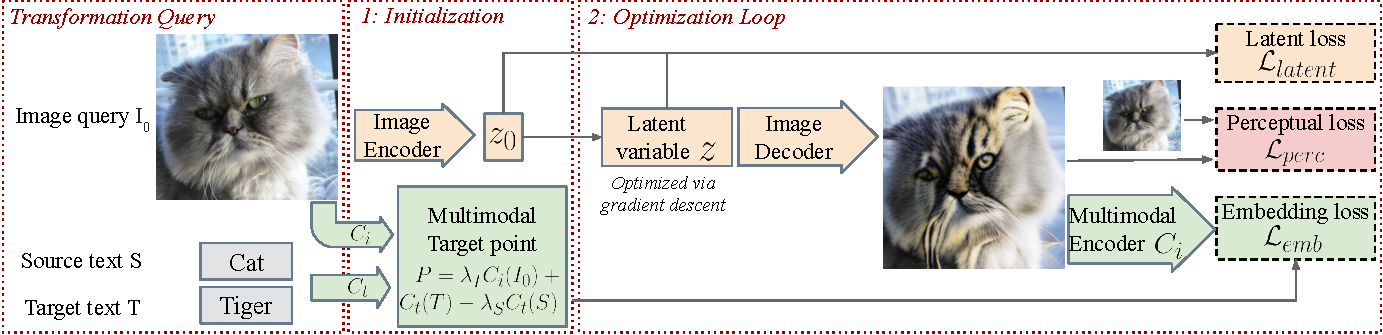
\includegraphics[width=\linewidth]{images/flexit/assets/method.pdf}
    \caption{FlexIT optimization framework: components  involving the multimodal latent space  colored in green; those involving the 
    image latent space in yellow; those involving the LPIPS distance in pink. Given a transformation query $(I_0, S, T)$, we first
     compute a target point $P$ in the multimodal embedding space, and we encode $I_0$ in the image latent space to get $z_0$. Then, 
     for a fixed number of steps, we update the latent variable $z$ (initialized with $z_0$) to get closer to the target point $P$. 
    We  add two regularization terms: the LPIPS perceptual distance between the input image and the output image, and a latent distance
     between $z$ and $z_0$. All networks are frozen, only $z$ is updated.}
    \label{fig:flexit_method}
\end{figure*}


\minipar{Optimization scheme}
The core idea of the FlexIT method is to edit the input image in a latent space, 
guided by a high-level semantic objective defined in the multimodal embedding space.
 Let $E$ be the image encoder, $D$ the image decoder and $(C_t, C_i)$ the multimodal 
 encoders for text and image respectively. Given an input image $I_0$ and a textual 
 transformation $S \rightarrow T$, we first initialize \ours by computing the initial 
 latent image representation as $z_0 = E(I_0)$ and the target multimodal point $P$ as
\begin{equation} 
P = C_t(T) + \lambda_{I} C_i(I_0) - \lambda_S C_t(S). \label{eq:p}
\end{equation}
We choose to use a multimodal embedding space since it allows text and image modalities 
to be combined together in a meaningful way: semantic transformations defined by textual
 embeddings can be applied to images with linear operations \citep{jia2021scaling}. In 
 this context, our target point $P$ can be seen as an image embedding that has been
  semantically modified with textual embeddings, by removing the source class information ($-\lambda_S C_t(S)$) 
  and adding the target class information ($+C_t(T)$). Since we don't know what is the optimal linear 
  combination of image and text embeddings, we consider $\lambda_I$ and $\lambda_S$ as parameters
   which will be validated on our development set.

To find an output image which, when encoded in the multimodal embedding space, gets as close as 
possible to the target point, we optimize the embedding loss: 
\begin{equation}
    \mathcal{L}_{emb}(z) = \Vert C_i(D(z)) - P \Vert_2^2.
\end{equation}


We add two regularization terms to the embedding loss, to encourage that only the content related to the transformation query is changed. 
Without regularization, the optimization scheme can alter any part of the image if this helps in getting closer to the multimodal target point, which we have found to yield unnatural artifacts. 
The distance to the input image $I_0$ is controlled with a LPIPS distance:
\begin{equation}
\mathcal{L}_{perc}(z) = d_{\text{LPIPS}} (D(z), I_0). 
\end{equation}

To enforce staying in parts of the latent space that are well decoded by our image decoder, we use a regularization term with respect to the initial latent code $z_0$. 
We use a $\ell_2$ norm at each spatial position $i$ of the latent code, and sum these norms across  spatial positions to obtain the loss: %a mixed $\ell_{2,1}$ norm:
\begin{equation}
\mathcal{L}_{latent}(z) = \sum_i \Vert z^i - z_0^i \Vert_2.
\end{equation}
This loss encourages sparse $z^i$ changes, \textit{i.e.}\ limiting changes in spatial locations, which is aligned with our 
objective to transform a localized part of the input image.

Finally, note that  $\lambda_I$ in Eq.\ (\ref{eq:p}) also acts as a regularization parameter, by encouraging  the input  and 
output image to be close in the multi-modal embedding space.

The total loss we optimize can be written as:
\begin{equation}
\mathcal{L}_{total}(z) = \mathcal{L}_{emb}(z) + \lambda_p \mathcal{L}_{perc}(z)  + \lambda_z \mathcal{L}_{latent}(z).
\end{equation}
After initialization, 
the latent image variable $z$ is updated via gradient descent with a fixed learning rate $\mu$ for a fixed number of steps $N$, 
while keeping all network weights frozen. Following the implementation of the Fast Gradient Method~\citep{dong2018boosting}, 
we normalize the gradient before the update.




\begin{figure}
    \centering
    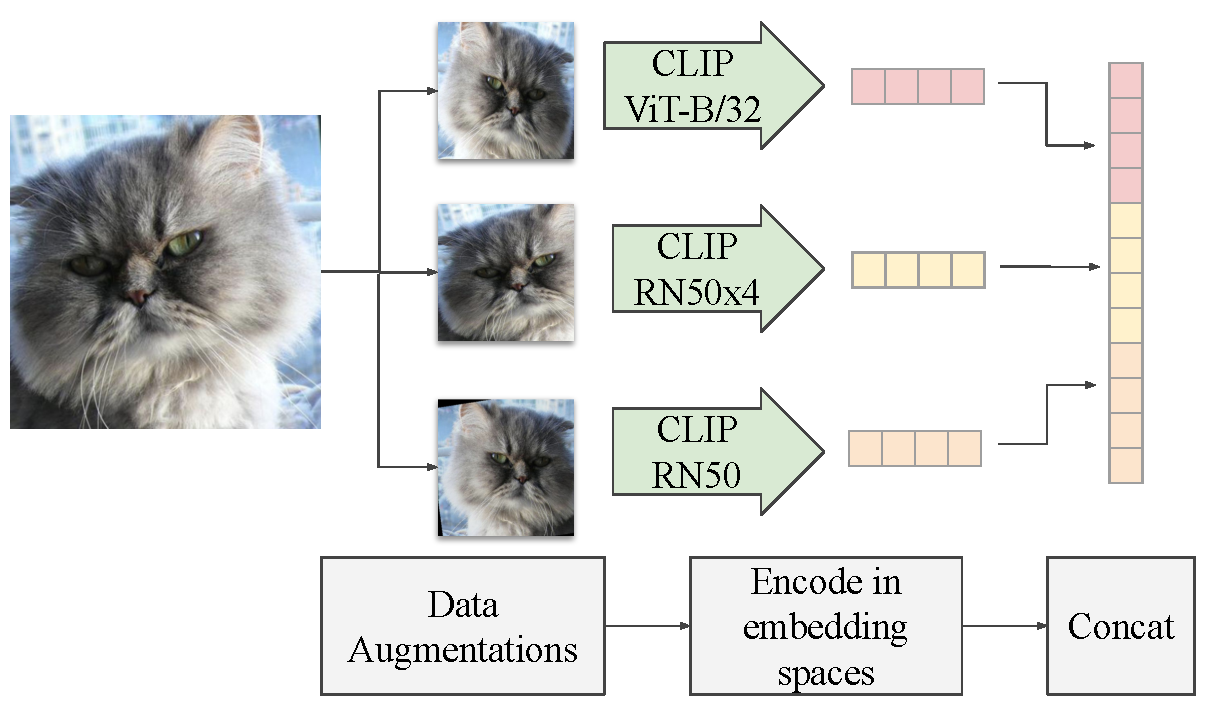
\includegraphics[width=\linewidth]{images/flexit/assets/clips.pdf}
    \caption{
    Architecture of our robust \ac{CLIP}-based image encoder, which combines three different  encoders by concatenation.}
    \label{fig:clips}
\end{figure}


\minipar{Image optimization space}
The distance to the multi-modal target point is a differentiable loss that can be 
optimized via gradient descent. A straightforward approach consists in performing
 gradient descent directly in the pixel-space. However, this type of image 
 representation lacks a  prior on low-level image statistics. 
By optimizing over a  latent variable instead, the  image is obtained as the
 output of a neural-network based decoder. Choosing an autoencoder, like that of 
 VQGAN, lets us (i) make use of the decoder's low-level priors, which guides the 
 optimization problem towards images that exhibit at least low-level consistency;
  and (ii) encode and decode images in its latent space with little distortion. 
  The spatial dimensions in the VQ-GAN latent space allows to edit specific parts
   of the image independently, contrary to \ac{GAN}s which typically rely on more global 
   latent variables. 
Although \ac{GAN}s generate realistic images with stronger priors, it is problematic to
 optimize their latent space for two reasons: first, \ac{GAN}s work  well on narrow 
 distributions (such as human faces), but do not work as well when trained  on a much 
 wider distribution;
second, even with a \ac{GAN} trained on a wide distribution such as that of ImageNet, it
 is hard to faithfully reconstruct  an image using its  latent space.

We report on experiments with optimization over raw pixels and \ac{GAN} latent spaces in  
Section~\ref{ablations}.



\section{Experimental Setup}


\subsection{Implementation details}\label{sub_section:implementation_details}

In \ours, we run the optimization loop for $N=160$ steps, which we found enough to 
transform most images. We use a resolution of 288 for encoding images with VQ-GAN,
 which compresses the images in a latent space with dimensions (256, 18, 18). 

We take advantage of  various pre-trained \ac{CLIP} models, and combine their embeddings
 with concatenation, as shown in Figure~\ref{fig:clips}. 

For the \ac{CLIP}-based multimodal encoders, we have considered all \ac{CLIP} networks freely available, listed in Table~\ref{tab:clip}.
 
\begin{table}[H]
\center
\begin{tabular}{lcc}
\toprule
\textbf{Backbone} & \textbf{Params.} & \textbf{Latent dim.}\\
\midrule
RN50 & 38M & 512\\
RN50x4 & 87M & 640\\
ViT-B/32 & 88M & 512\\
ViT-B/16 & 86M & 512 \\
RN50x16 & 167M & 768\\
\bottomrule
\end{tabular}
\caption{Visual backbones used for the multimodal encoder. Our default configuration only includes the ViT-B/32, the RN50 and the RN50x4.}
\label{tab:clip}
\end{table}

By default, we use three image embedding networks with two different ResNets  and one \ac{ViT} 
architectures, which implement complementary inductive biases.

To encode an image with a single \ac{CLIP} network, we average the embeddings of multiple
 augmentations of the input image. 
 For data augmentations, we use a random horizontal flipping and a random rotation between $-10$ and $10$ degrees, 
 followed by cropping the image (keeping at least $80\%$ of the input image) with aspect ratio between $0.9$ and $1.1$.


For the regularization coefficients, we use 
$\lambda_z=0.05,$ $\lambda_p = 0.15,\ \lambda_S=0.4,\ \lambda_I = 0.2$ as our 
default values. 
These coefficients are set using 
our ImageNet-based development set, and are fixed for all experiments. 


These implementation choices are analysed in Section~\ref{hparam}.



\subsection{Evaluation dataset} 
We did not find a satisfying evaluation framework to study the problem of semantic image
 translation: existing dataset and metrics focus on narrow image domains, or random text
  transformation queries~\citep{li2020manigan,patashnik2021styleclip}. 

To overcome this, we have decided to build upon the ImageNet dataset~\citep{deng2009imagenet}
 for its diversity and its high number of classes: by defining which class labels can be
  changed into one another (like \textit{cat} $\rightarrow$ \textit{tiger}), we can
   build a set of sensible object-centric transformation queries. 

We have selected a subset of the 273 ImageNet labels that we manually split into 47 
clusters according to their semantic similarity as given by the WordNet hierarchy of classes.
For instance, there is a cluster 
containing all kinds of vegetables. 
The resulting clusters are shown in Table~\ref{fig:clusters}. 
 We have not included all ImageNet classes 
because (i) we wanted to reduce the large number of dog breed classes, and (ii) a 
lot of classes were ``standalone classes'' with no natural target for transformation 
among the other classes.

%
We only consider  transformations  $S \rightarrow T$ where $S$ and $T$ are in the same 
cluster, in order to avoid nonsensical transformations between unrelated objects, \eg 
laptop $\rightarrow$ butterfly.

For each target label $T$ we construct eight transformation queries by randomly 
sampling eight other classes $\{S_i\}$ within the same cluster, and sample a random 
image from each $S_i$ from the ImageNet validation set.
This gives  a total of 2,184 transformation queries that we split into a development
 set and a test set of equal size.
We use the development set to tune various hyper-parameters of our approach, and 
report evaluation metrics on the test set.


\renewcommand\cellgape{\Gape[1pt]}
\begin{table*}
\footnotesize
\center
\begin{tabular}{lll}
\toprule
\thead[l]{Group} & \thead[l]{Cluster} & \thead[l]{Classes} \\
\midrule
bird & bird of prey & bald eagle, kite, great grey owl \\
bird & finch & indigo bunting, goldfinch, house finch, junco \\
bird & grouse & black grouse, prairie chicken, ptarmigan, ruffed grouse \\
bird & seabird & king penguin, albatross, pelican, European gallinule, black swan \\
bird & wading bird & goose, oystercatcher, little blue heron, black stork, bustard, flamingo, spoonbill \\
\midrule
container & bag & backpack, plastic bag, purse \\
container & food container & \makecell[l]{water jug, beer bottle, water bottle, wine bottle, coffee mug, vase, \\coffeepot, teapot, measuring cup, cocktail shaker} \\
\midrule
device & electronics & \makecell[l]{cassette player, cellular telephone, computer keyboard, desktop computer, \\dial telephone, hard disc, iPod, laptop} \\
device & measuring & analog clock, digital clock, wall clock, stopwatch, digital watch, odometer, barometer \\
\midrule
dog & hound & English foxhound, Italian greyhound, Afghan hound, basset, beagle, otterhound \\
dog & sporting dog & English springer, cocker spaniel, golden retriever, Irish setter \\
dog & terrier & \makecell[l]{American Staffordshire terrier, wire-haired fox terrier, standard schnauzer, \\Border terrier, Irish terrier, Yorkshire terrier} \\
dog & toy dog & papillon, Chihuahua, Japanese spaniel, Shih-Tzu, toy terrier \\
dog & working dog & \makecell[l]{collie, German shepherd, Rottweiler, miniature pinscher, \\French bulldog, Siberian husky, boxer, Eskimo dog} \\
\midrule
edible & edible fruit & Granny Smith, strawberry, lemon, orange, banana, custard apple, fig, pineapple, pomegranate \\
edible & sandwich & cheeseburger, hotdog, bagel \\
edible & vegetable & \makecell[l]{bell pepper, broccoli, cauliflower, spaghetti squash, zucchini, \\butternut squash, artichoke, cardoon, cucumber} \\
\midrule
fungus & fungus & bolete, coral fungus, earthstar, gyromitra, hen-of-the-woods, stinkhorn \\
\midrule
insect & beetle & ground beetle, ladybug, leaf beetle, long-horned beetle, tiger beetle, weevil \\
insect & butterfly & monarch, admiral, cabbage butterfly, lycaenid, ringlet, sulphur butterfly \\
insect & spider & black widow, garden spider, tarantula, wolf spider, scorpion \\
\midrule
mammal & bear & American black bear, brown bear, ice bear, sloth bear, giant panda, lesser panda \\
mammal & bovid & ox, ibex, bighorn, gazelle, impala, water buffalo, ram, bison \\
mammal & canine & \makecell[l]{Arctic fox, grey fox, red fox, African hunting dog, dingo, \\coyote, red wolf, timber wolf, white wolf, hyena} \\
mammal & equine & sorrel, zebra \\
mammal & feline & Persian cat, tabby, cheetah, jaguar, leopard, lion, snow leopard, tiger \\
mammal & great ape & chimpanzee, gorilla, orangutan \\
mammal & monkey & capuchin, spider monkey, squirrel monkey, baboon, guenon, macaque \\
\midrule
music. instr. & percussion & chime, drum, gong, maraca, marimba, steel drum \\
music. instr. & stringed & cello, violin, acoustic guitar, electric guitar, banjo \\
music. instr. & wind & bassoon, oboe, sax, flute, cornet, French horn, trombone \\
\midrule
object & ball & golf ball, ping-pong ball, rugby ball, soccer ball, tennis ball \\
object & handtool & hammer, plane, plunger, screwdriver, shovel \\
object & headdress & bathing cap, shower cap, bonnet, cowboy hat, sombrero, football helmet \\
\midrule
reptile & amphibian & bullfrog, tree frog, axolotl, spotted salamander, common newt, eft, European fire salamander \\
reptile & snake & \makecell[l]{rock python, boa constrictor, green mamba, Indian cobra, diamondback, sidewinder, \\horned viper, king snake, green snake, thunder snake} \\
reptile & turtle & box turtle, mud turtle, terrapin \\
\midrule
sea life & aqu. mammal & killer whale, grey whale, sea lion, dugong \\
sea life & bony fish & goldfish, tench, eel, anemone fish, lionfish, gar, sturgeon \\
sea-life & crab & American lobster, Dungeness crab, fiddler crab, king crab, rock crab, crayfish, hermit crab, isopod \\
sea life & shark & great white shark, tiger shark, hammerhead \\
\midrule
vehicle & bicycle & motor scooter, tricycle, unicycle, mountain bike, moped \\
vehicle & boat & speedboat, lifeboat, canoe, fireboat, gondola \\
vehicle & car & ambulance, beach wagon, cab, convertible, jeep, limousine, minivan, sports car \\
vehicle & locomotive & electric locomotive, steam locomotive \\
vehicle & sailing vessel & catamaran, trimaran, schooner \\
vehicle & truck & minivan, police van, fire engine, garbage truck, pickup, tow truck, trailer truck, school bus \\
\bottomrule
\end{tabular}

\caption{Groups and clusters of the ImageNet classes used to define the transformation queries.
}
\label{fig:clusters} 
\end{table*}


For results, we report quantitative and qualitative results for images from the ImageNet test set. 
We also show  qualitative results from the Stanford Cars dataset~\citep{KrauseStarkDengFei-Fei_3DRR2013}.
Finally, we also show that our method can used on any image in-the-wild, with the image of a 
sow's ear on Figure~\ref{fig:main_demo}.


\subsection{Metrics}
%
We  evaluate the success of the transformation by means of the \textbf{Accuracy} of an 
image  classifier, which is possible since we use ImageNet class labels as the 
transformation targets.
%
We use a DeiT \citep{touvron2021deit} classifier, which has an ImageNet validation 
accuracy of 85.2\%. 
We judge a transformation  successful if, for the transformed image, class $T$ has
 the highest  probability among the  273 selected classes.
The classifier takes images of size 384$\times$384. Smaller images are upsampled before 
being passed to the classifier.

To assess naturalness of  transformed images, we use the \ac{FID}~\citep{heusel2017gans}.
In particular, because we use a small number of samples, we use the (\textbf{\ac{SFID}}).
In addition to the \ac{SFID}, we use a class-conditional
 SFID score  (\textbf{CSFID}) which is an average of the \ac{SFID} scores computed for each 
 target class separately.
  Please refer to \ref{sec:related_fid} for a detailed description these metrics. 
 Because we compute these scores with a low number of examples 
  for many classes, the \ac{CSFID} score has a high bias, low variance profile on our
   dataset \citep{chong2020effectively}, and we  
 have found it to be reliable and stable. We have noticed that the distance on standard deviations was not very discriminative: 
 since we are modifying images and not generating images from scratch, we already have
  a lot of diversity in the generated images. 
  Experimentally, using $\alpha > 0$ of Equation~\ref{{eq:sfid}} mostly consisted in
   adding a bias term in this metric, therefore we chose to use $\alpha =0 $ in the (C)SFID scores. 

Since the images we transform are extracted from the ImageNet validation set, we use the ImageNet training set as our 
reference distribution to compute the (C)SFID scores. 
The (C)SFID scores are computed at an image resolution of 256.



The \ac{CSFID} metric is a measure of both image quality and transformation accuracy, as it 
measures the feature distribution distance between the transformed images and the 
reference images from the target class in the %ImageNet 
training set. 
Editing should not change parts of the image that are irrelevant to the transformation
 defined in the text,  \eg the background.  
We use the \textbf{LPIPS} perceptual distance~\citep{zhanglpips2018}  to measure deviation 
from the input image (see \ref{sec:related_lpips}). 
As recommended by the authors, we use the AlexNet~\cite{krizhevsky12nips} backbone to 
compute \ac{LPIPS} distance, when we use it as
an evaluation metric. During training, so as to reduce bias in the \ac{LPIPS} evaluation, we used the 
\ac{LPIPS} distance based on VGG features.

The \ac{LPIPS}  distance is computed at an image resolution of 256, for both evaluation and 
optimization.
All \ac{LPIPS}  scores which we will present have been multiplied by 100 for readibility.

The \ac{LPIPS}  distance cannot distinguish edits which are relevant to the text 
query from those which are not; and we don't know the minimal \ac{LPIPS} distance between 
an image and its closest successful transformation. Still, we argue that it should be 
as low as possible.


\subsection{Baselines}
We consider two extreme configurations as baselines,  which only optimize one of these 
two criteria: (i) The  \textsc{Copy} baseline, which simply copies the input image
 without any modification,
and  (ii) the \textsc{Retrieve} baseline that outputs a random validation image 
labelled with the target class $T$.
We add the \textsc{Encode} baseline that simply passes the input image through the 
VQ-GAN autoencoder. 
We also evaluate  StyleCLIP~\citep{patashnik2021styleclip}, the most relevant 
text-driven image transformation algorithm from the literature. We consider the 
version most similar to our method that embeds images with an ImageNet-trained 
StyleGAN2 (see source in next section). We train our own e4e encoder~\cite{tov2021designing} 
to embed images into this latent space.
StyleCLIP iteratively updates the StyleGAN2 latent representation to maximize the similarity
  with a given text in the \ac{CLIP} latent space. Finally, we evaluate
  ManiGAN~\citep{li2020manigan}, which we have trained on ImageNet with the  implementation from the authors.

\subsection{Assets}

We provide a list of the assets used in our work (datasets, code, and models) in
the Appendix in~\ref{sec:FlexIt assets}.


\section{Qualitative Results}


Qualitative results of FlexIT transformations on ImageNet images are presented in 
Figures~\ref{fig:main_demo} and ~\ref{fig:visuresu}.
Figure~\ref{fig:visuresu} shows successful transformations as well as several
 failure cases. 
To demonstrate the generality of our approach, we also  show examples of color 
transformations for images from the Stanford Cars 
dataset~\citep{KrauseStarkDengFei-Fei_3DRR2013} in Figure~\ref{fig:cars30k}.


\begin{figure}
    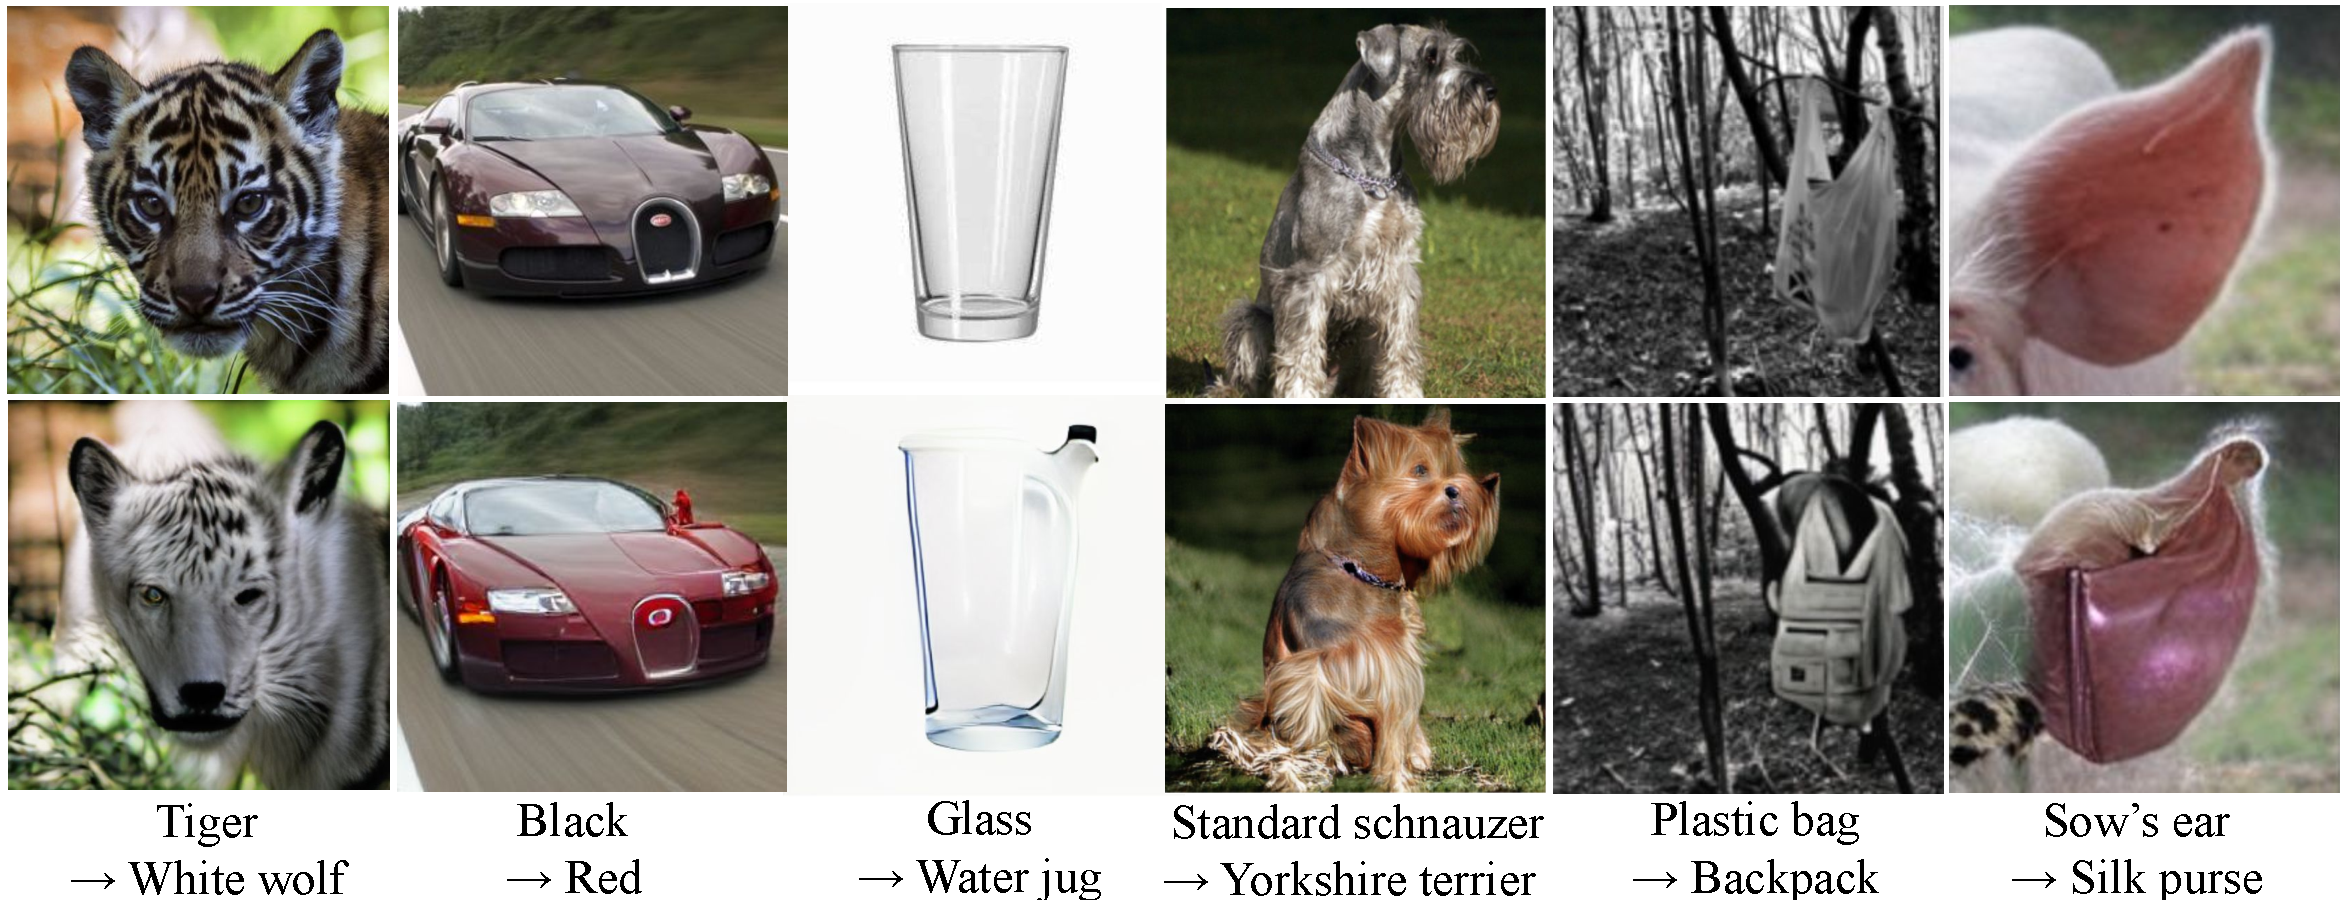
\includegraphics[width=\textwidth]{images/flexit/assets/demo1.pdf}
    \captionof{figure}{\ours transformation examples. From top to bottom: input image, transformed image, and text query.
    }
    \label{fig:main_demo}
\end{figure}

\begin{figure*}
    \centering
    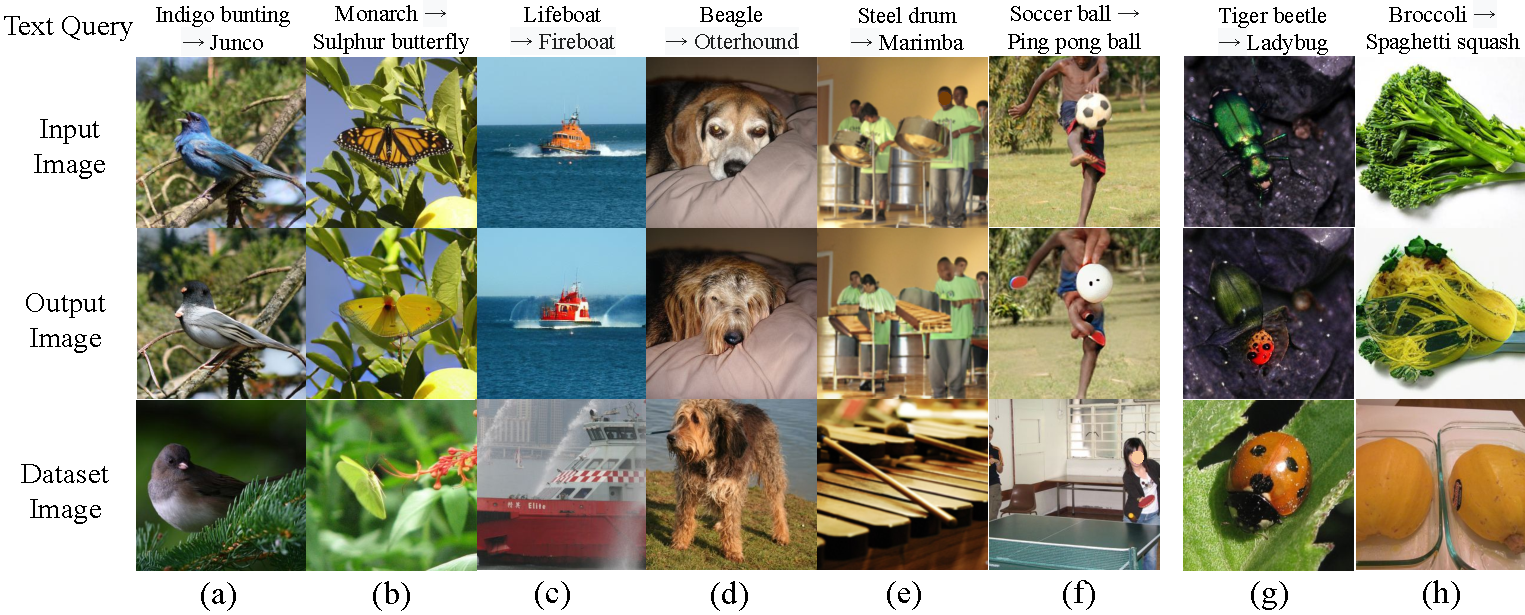
\includegraphics[width=\linewidth]{images/flexit/assets/main_exs.pdf}
    \caption{Transformation examples with \ours on ImageNet images. 
    From top to bottom: input and output image, as well as dataset image from the target
     class.
    Columns (a)-(e) show examples of successful transformations. Column (f) shows an
     interesting behavior where another object has been added in the image to add more 
     context (a table tennis racket in the hand of the person). The  last two columns 
      show the most frequent modes of failure: only part of the input object is
       transformed (g), or parts of the input object that should be changed are not 
       changed: in column (h), the transformed images still has a broccoli shape with 
       green parts instead of an orange and round spaghetti squash.
    }
\label{fig:visuresu}
\end{figure*}


\begin{figure}
    \centering
    \vspace{-1em}
    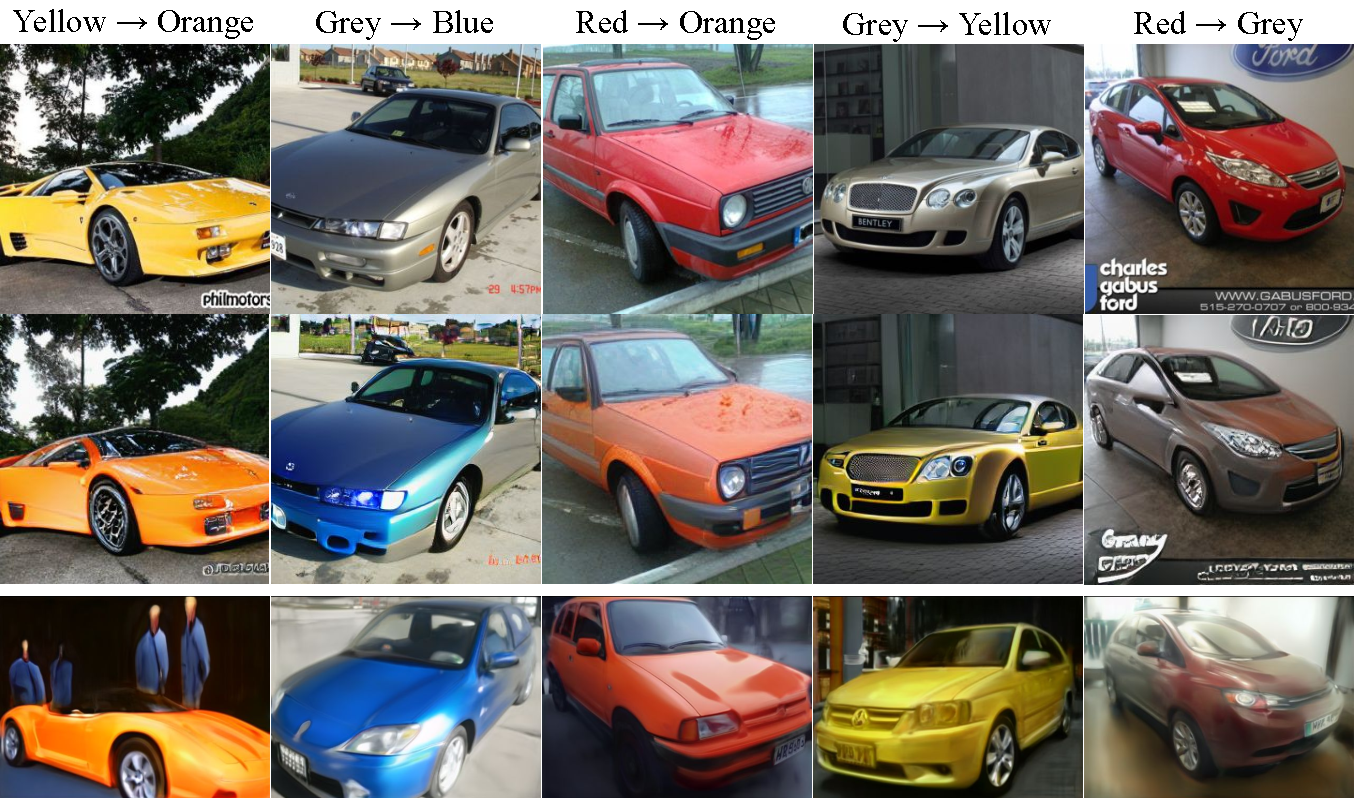
\includegraphics[width=\linewidth]{images/flexit/assets/cars2.pdf}
    \caption{Example  transformations on the \textit{Cars} dataset:  input images (first row),  \ours results  (second row), StyleCLIP results based on a  StyleGAN2 backbone pre-trained on LSUN Cars.
    dataset (last row). Although GAN-based images have better details like the wheels, they are farther away from the input images.}
    
    \label{fig:cars30k}
\end{figure}

Finally, Figure~\ref{fig:steps} shows intermediate transformation results with FlexIT for 0, 8, 16, 32 and 160 optimization steps. 
The result after zero optimization steps shows the effect of autoencoding the input image, without changing the latent representation.

\begin{figure*}[t!]
    \center
    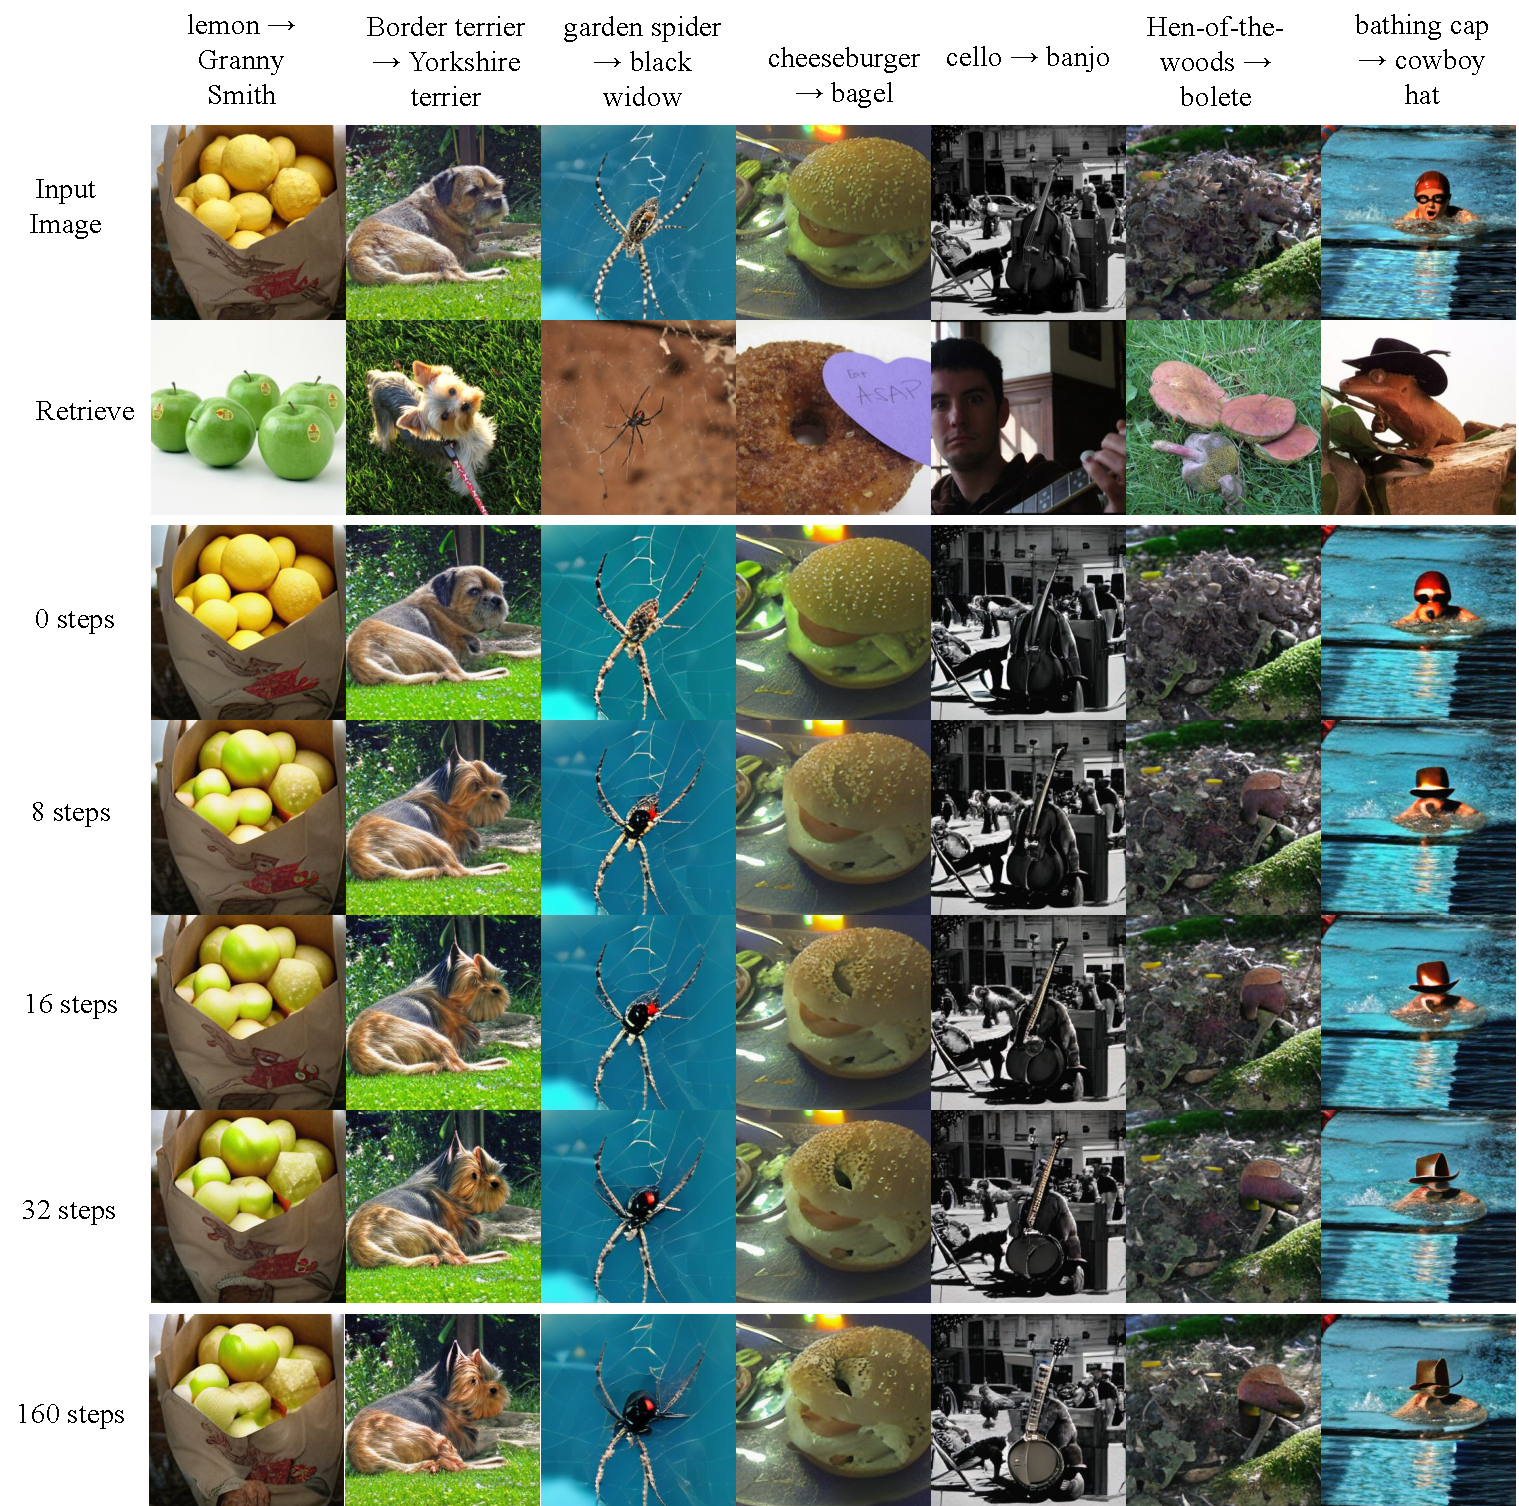
\includegraphics[width=\linewidth]{images/flexit/assets/steps.pdf}
    \caption{Intermediate transformation results obtained with FlexIT. Note that most edits only require 32 steps to be completed; some edits benefit from longer optimization schemes, such as the  spider and the banjo.
    }
    \label{fig:steps}
\end{figure*}

\section{Quantitative Results}

Semantic image translation is inherently a trade-off between having the most relevant 
and natural output image (as measured by Accuracy, \ac{CSFID} and \ac{SFID}), while staying as 
close as possible to the input image (as measured by \ac{LPIPS}). 

Results are reported in Table~\ref{tab1}. 
As expected, the copy baseline is ideal on \ac{LPIPS} and \ac{SFID}, but fails to adapt to the 
transformation target $T$, and thus fails on Accuracy and \ac{CSFID}.
For the same reason, the auto-encoding baseline also fails on Accuracy and \ac{CSFID}, but 
demonstrates the non-trivial impact of using the VQ-GAN latent space on \ac{LPIPS} and \ac{SFID}. 
The \textsc{Retrieve} baseline provides ideal metrics for Accuracy, \ac{CSFID} and \ac{SFID}, as 
it returns natural images of the target class. 
It fails  on \ac{LPIPS}, however, since the output image is unrelated to the input. 


\begin{table}
\centering
\small
\resizebox{\columnwidth}{!}{
\begin{tabular}{lrrrr}
\toprule
& \thead{LPIPS ↓} & \thead{Acc.\%↑} & \thead{CSFID ↓} & \thead{SFID ↓}  \\
\midrule
\textsc{Copy} & 0.0 & 0.45 & 106.0 & 0.2 \\
\textsc{Encode} & 17.5 & 1.6 & 107.5 & 3.0 \\
\textsc{Retrieve} & 72.4 & 90.6  & 27.2 & 0.2 \\
%ManiGAN~\cite{li20cvpr}    & ? & ? & ? & ? \\
ManiGAN~\cite{li2020manigan} & 21.7 & 2.0 & 123.8 & 17.0 \\ 

StyleCLIP~\cite{patashnik2021styleclip} & 33.4 & 8.0 & 146.6 & 35.8 \\ 
%StyleCLIP+1,000~\cite{patashnik2021styleclip}   
\ours (Ours) & 24.7 & 51.3 & 57.9 & 6.8 \\
\bottomrule
\end{tabular}}
\caption{Evaluation  of \ours and baselines on ImageNet images. %, comparing to baselines and StyleCLIP. 
}
\label{tab1}
\end{table}
%lpips=33.435783. acc=8.058608	csfid=146.609222	sfid=35.824425	




Our \ours approach  combines a  low \ac{LPIPS} (24.7 \vs 17.5 for \textsc{Encode}) with an 
accuracy of 51.3\% and a \ac{CSFID} of 57.9, which is closer to the \ac{CSFID} of
\textsc{Retrieve} (27.2) than that of \textsc{Encode} (107.5).
The StyleCLIP scores are poor, with high \ac{SFID} and \ac{CSFID} scores which was expected as 
StyleCLIP has been designed to work well where GANs shine.
The StyleGAN2 model we use, trained on ImageNet, is agnostic to class information and 
cannot synthesize realistic images for all ImageNet classes.
ManiGAN works well when trained on narrow domains with color change transformation 
requests, but we find that it does not produce convincing edits when trained on 
ImageNet.

\begin{figure}
    \centering
    \vspace{-1em}
    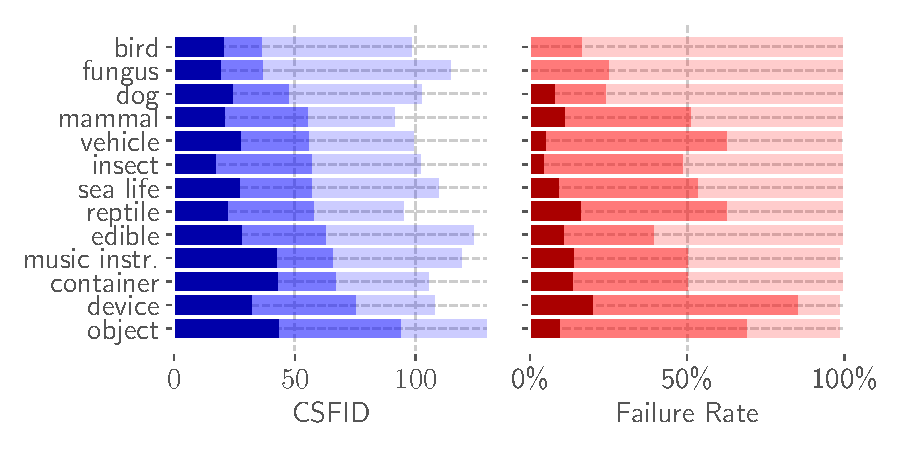
\includegraphics[width=\linewidth]{images/flexit/assets/classwise.pdf}
    \caption{Groupwise CSFID  and Failure Rate (1-Accuracy),  lower is better for both metrics. 
    Dark colors: best possible values obtained with  \textsc{Retrieve} baseline; medium colors: scores obtained with \ours; light colors: values obtained with  \textsc{Copy} baseline. 
    }
    
    \label{fig:classwise}
\end{figure}

To provide insight into which transformations work well, and which less so, we group 
our 47 ImageNet clusters into 13 bigger groups and report 
the average \ac{CSFID} and failure rate ($1 -$accuracy) scores for each group in Figure~\ref{fig:classwise}.
Generally, transformations among  natural objects are more successful than
 transformations among man-made objects. We believe that this is mostly because the 
 latter appear in a wider variety of shapes and contexts which leads to more difficult 
 transformations.


We argue that our evaluation protocol is well-suited for evaluating text-driven image editing because it 
(1): offers a list of sensible transformation queries and (2) offers a method for evaluating the quality and accuracy 
of the generated result. However, to further compare to ManiGAN~\citep{li2020manigan}, we propose to compare our method 
while following their 
evaluation protocol used in their paper. This consists in using the COCO dataset and (1) choosing 
\textit{random} COCO captions/image pairs and thus leading to noisy transformations and (2) calculating the image-text similarity
 score which was used as a loss term during their training, leading to bias in the final scores.
 We show 
 in Tab.\ \ref{results_manigan} that even with this COCO evaluation, FlexIT improves upon the scores of ManiGAN by a large margin.

\begin{table}[H]
\small
\centering
\begin{tabular}{l|l|l|l|l|}
\cline{2-5}
                              & \multicolumn{1}{c|}{IS↑} & \multicolumn{1}{c|}{SIM↑} & \multicolumn{1}{c|}{DIFF↓}             & \multicolumn{1}{c|}{MP↑} \\ \hline
\multicolumn{1}{|l|}{ManiGAN} & 14.96                   & 0.087                    & 0.216                                 & 0.068                   \\ \hline
\multicolumn{1}{|l|}{FlexIT}  & \textbf{18.19}          & \textbf{0.177}           & {\color[HTML]{000000} \textbf{0.146}} & \textbf{0.151}          \\ \hline
\end{tabular}
\caption{ManiGAN evaluation on random transformation requests from COCO.}
\label{results_manigan}
\end{table}


\section{Ablation studies\label{ablations}}


\begin{figure}
    \centering
    \vspace{-1em}
    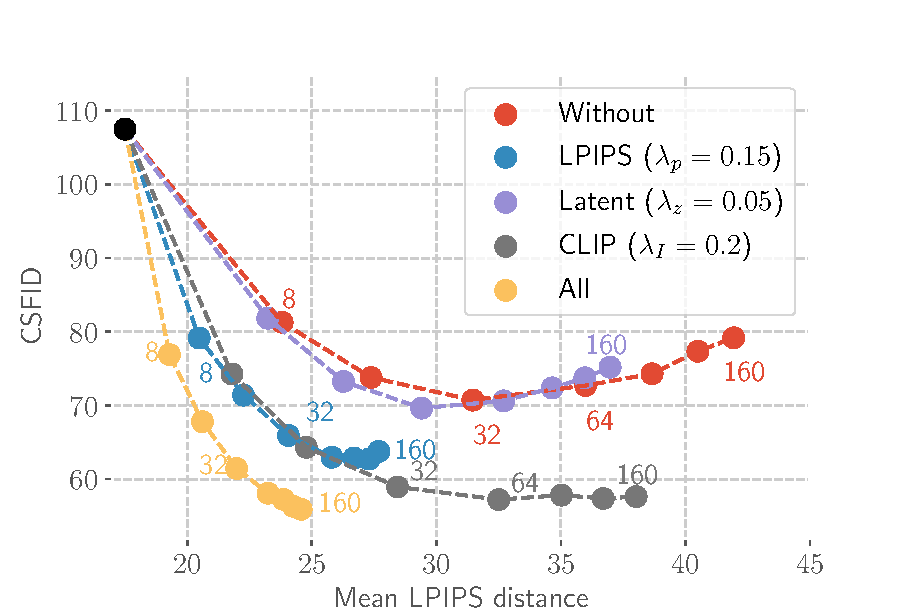
\includegraphics[width=\linewidth]{images/flexit/assets/reg_evol.pdf}
    \caption{\ac{CSFID} obtained without regularization, with individual \ac{LPIPS}, Latent and \ac{CLIP} regularizers, and using all. 
    Each curve corresponds to 160 steps of optimization on the dev.\ set. 
    }
    \label{fig:regul}
\end{figure}

\subsection{Regularizers}
In Figure~\ref{fig:regul}, we show the evolution of \ac{CSFID} along the optimization steps, 
where we consider our method without regularization, with each regularization scheme 
separately, and with all regularizers (default configuration).
Compared to not using regularization, the \ac{LPIPS} regularization substantially improves
 the \ac{CSFID} score along the optimization path, while also reducing \ac{LPIPS} as expected. 
The \ac{CLIP} regularizer has a similar effect, but is able to reduce  \ac{CSFID} further while
 the \ac{LPIPS} distance is only slightly reduced compared to our method without any 
 regularization.
%We believe that 
These two regularizers are complementary: while the \ac{LPIPS} loss mitigates image 
deviation for local features, the \ac{CLIP} loss provides semantic guidance which helps to 
reconstruct recognizable objects. %details like faces.
Using all regularizers allows us to obtain the lowest \ac{CSFID} scores at low \ac{LPIPS}. 
Corresponding qualitative examples are shown in Figure~\ref{fig:demo_reg}. 

\begin{figure}
    \centering
    \vspace{-1em}
    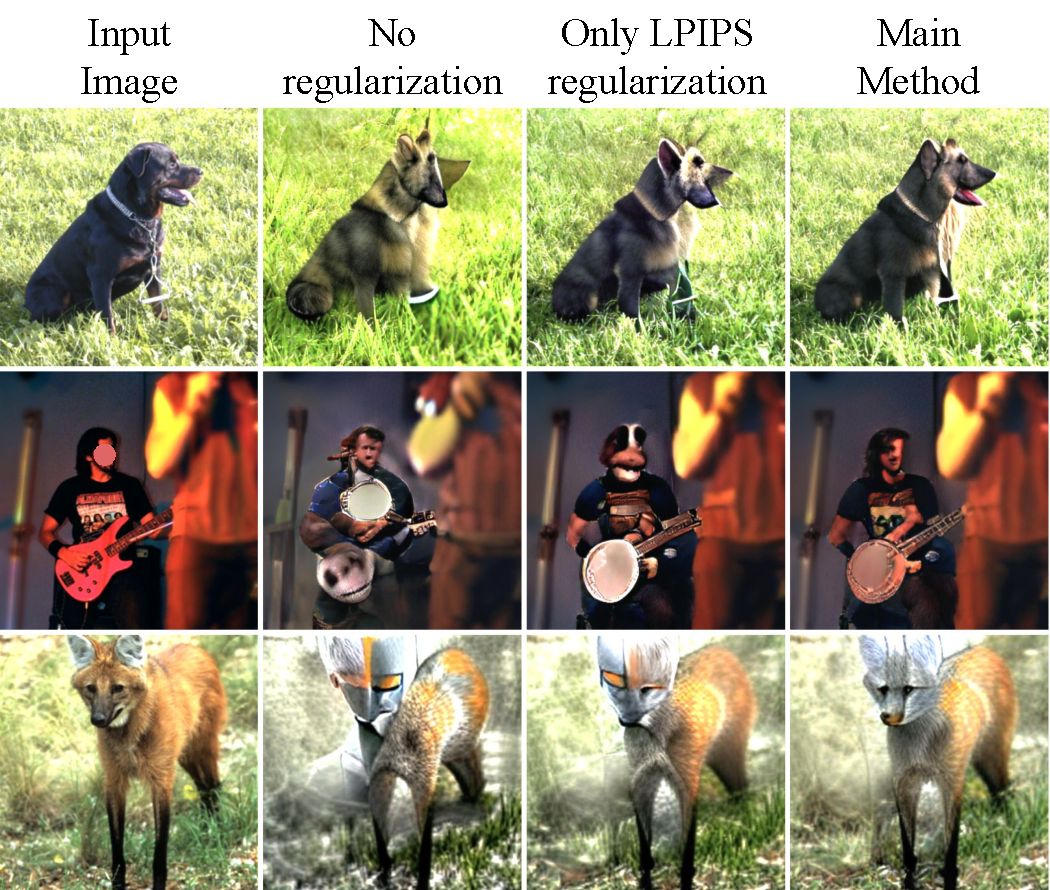
\includegraphics[width=\linewidth]{images/flexit/assets/demo_reg2.pdf}
    \caption{Example transformations with different regularizers. Textual queries from top to bottom: Rottweiler → German shepherd, Electric guitar → Banjo, Red wolf → Grey fox.
    }
    \label{fig:demo_reg}
\end{figure}


\begin{figure}
    \centering
    \vspace{-1em}
    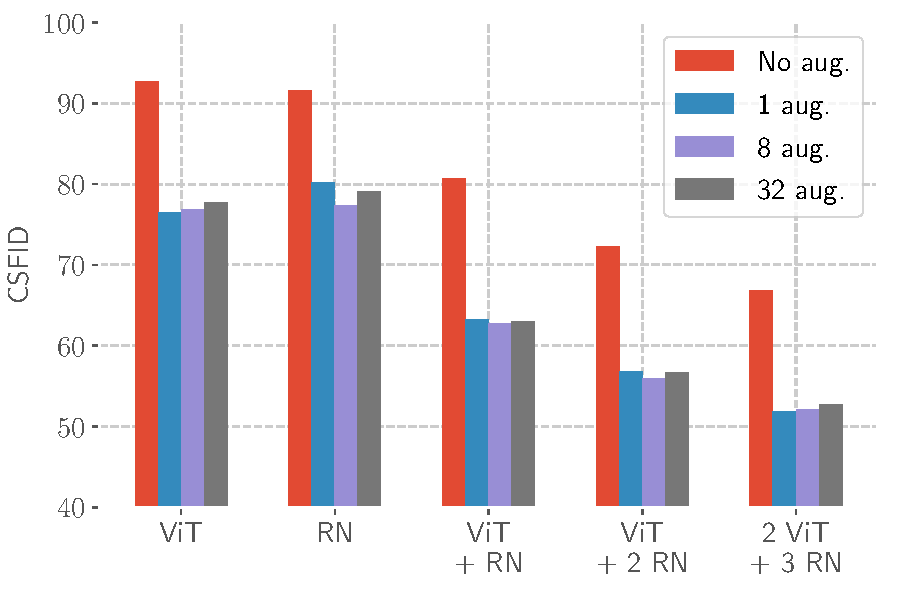
\includegraphics[width=.9\linewidth]{images/flexit/assets/naug_nnets.pdf}
    \caption{CSFID for different CLIP networks combinations and number of data augmentations options. Default setting: ViT+2RN.}
    \label{fig:augs}
    \vspace{-1em}
\end{figure}


In Table~\ref{table:ablations}, we detail the ablation experiments for all FlexIT parameters.

\begin{table}
\small
\center
\begin{tabular}{lrrrr}
\toprule
 & \textbf{Acc.↑} & \textbf{LPIPS↓} & \textbf{CSFID↓} & \textbf{SFID↓} \\
\midrule
                   $\lambda_I=0$ & \textbf{64.8} &   27.6 &   65.4 & 12.3 \\
                   $\lambda_I=0.1$ & 60.6 &   25.9 &   57.8 &  8.3 \\
                     
                    \rowcolor{LightGrey} $\lambda_I=0.2$   & 52.6 &   24.6 &   \textbf{55.9} &  6.4 \\
                   $\lambda_I=0.3$ & 45.8 &   23.5 &   56.3 &  5.5 \\
                   $\lambda_I=0.4$ & 38.6 &   \textbf{22.6} &   58.6 &  \textbf{5.0} \\
                   \midrule
                   $\lambda_S=0.0$ & 34.3 &   \textbf{23.8} &   60.2 &  \textbf{4.8} \\
                  $\lambda_S=0.2$ & 45.9 &   24.0 &   57.3 &  5.5 \\
                  \rowcolor{LightGrey} $\lambda_S=0.4$   & 52.6 &   24.6 &   \textbf{55.9} &  6.4 \\
                  
                   $\lambda_S=0.5$ & 56.2 &   25.0 &   56.5 &  7.1 \\
                   $\lambda_S=0.8$ & \textbf{60.0} &   26.5 &   65.5 & 11.7 \\
                   \midrule
                   $\lambda_z=0.0$ & \textbf{59.4} &   26.5 &   56.1 &  7.1 \\
                   \rowcolor{LightGrey} $\lambda_z=0.05$& 52.6 &   24.6 &  \textbf{55.9} &  6.4 \\
                   $\lambda_z=0.1$ & 51.0 &   \textbf{23.3} &   56.7 &  \textbf{6.3} \\
                   \midrule
                   $\lambda_p=0.05$ & \textbf{66.2} &  28.8 &  \textbf{56.0} &  7.9 \\
                   $\lambda_p=0.1$ & 59.1 &   26.4 &   \textbf{56.0} &  7.2 \\
                   \rowcolor{LightGrey} $\lambda_p=0.15$   & 52.6 &   24.6 &  \textbf{55.9} &  6.4 \\
                   $\lambda_p=0.2$ & 47.9 &   \textbf{23.3} &   57.5 & \textbf{6.3} \\
                   \midrule
                    $\ell_1$ & \textbf{54.2} &   \textbf{24.6} &   56.3 &  6.5 \\
                    $\ell_2$ & 52.4 &   \textbf{24.5} &  \textbf{55.9} &  6.8 \\
                    \rowcolor{LightGrey} $\ell_{2,1}$ & 52.6 &   \textbf{24.6} &  \textbf{55.9} &  \textbf{6.4} \\
                    \midrule
                    $lr=0.025$ & 47.6 &   \textbf{22.5} &   58.3 &  \textbf{6.0} \\
                    \rowcolor{LightGrey} $lr=0.5$     & 52.6 &   24.6 &    55.9 &  6.4 \\
                    $lr=0.1$ & \textbf{60.4} &   27.6 &   \textbf{54.8} &  7.2 \\
                    \midrule
                  resolution 256 & 53.8 &   24.8 &   56.8 &  7.2 \\
                  \rowcolor{LightGrey} resolution 288 & \textbf{52.6} &   24.6 &   \textbf{55.9} &  \textbf{6.4} \\
                  resolution 320 & 54.3 &   \textbf{24.0} &   57.4 &  7.3 \\
                  \bottomrule
\end{tabular}

\caption{\label{table:ablations} FlexIT ablation results. $lr$ is the learning rate. Lines corresponding to our default configuration are marked in light grey. The norms $\ell_1$,  $\ell_2$, and $\ell_{2,1}$  refer to the distance used for regularization in the VQ-GAN latent space. Best values for each metric are shown in bold inside each group of parameter values.
}
\end{table}


\subsection{CLIP embedding module and Data Augmentations} 
We study how different choices of \ac{CLIP} image encoders impact the \ac{CSFID} score. 
Our default configuration involves two ResNet-based networks and one ViT-based network 
to embed the image in the \ac{CLIP} space. 
We experiment with a single ViT or ResNet, a combination of ViT with a single  ResNet,  
and also using all available pre-trained \ac{CLIP} networks, which comprises a ViT-B/16, a
 ViT-B/32, a ResNet50, ResNet50$\times$4 and ResNet50$\times$16,
  see~\citep{radford2021learning} for details on the modules.
For each \ac{CLIP} network configuration, we experiment with  either  not using data 
augmentation, or using $d \in\{ 1, 8, 32\}$ augmentations, as described in~\ref{sub_section:implementation_details}.
Each of the $N_\textrm{nets}$ \ac{CLIP} networks sees a different augmentation in each of 
the $N_\textrm{steps}$ optimization steps,  resulting in a total of
 $d \times N_\textrm{nets} \times N_\textrm{steps}$ augmentations of the input image.

From the results in Figure~\ref{fig:augs}, we see that while the  ViT and  ResNet 
embedding networks lead to similar results, they are complementary and combining them 
leads to a substantial improvement.  
Adding additional networks leads to further improvements.
%
Second, using data augmentation is very beneficial, and leads to a reduction in \ac{CSFID} 
of 10 or more points for all network configurations. 
Using more than one augmentation does not improve results substantially: it suffices 
to use a different augmentation for each network at each optimization step.
In our other experiments we use the three smallest (and fastest) \ac{CLIP} networks as our 
default setting.


\begin{figure}
    \centering
    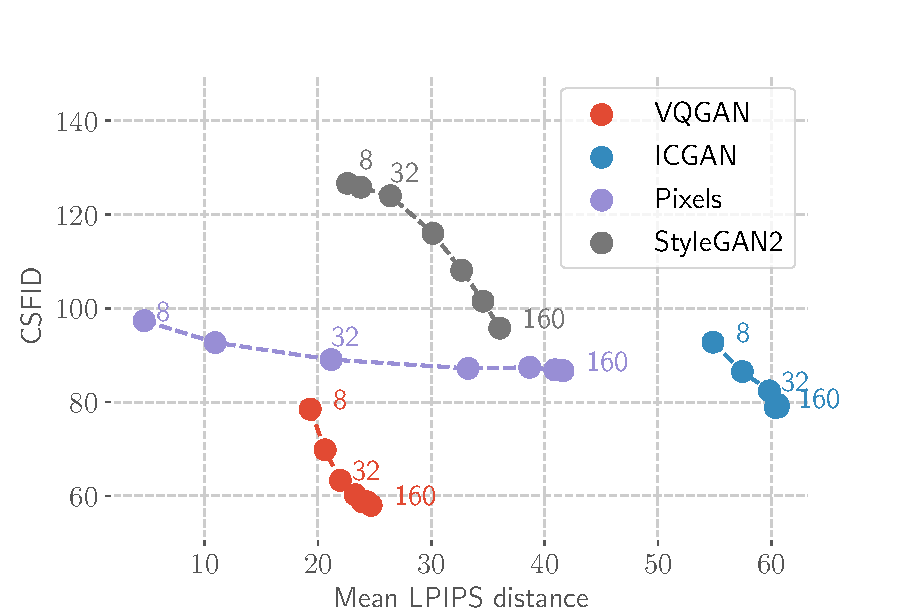
\includegraphics[width=.9\linewidth]{images/flexit/assets/encoder_evol.pdf}
    \caption{\ac{CSFID} and \ac{LPIPS} scores across iterations, using different latent spaces, or raw pixels, for optimization. 
    }
    \label{fig:encoders}
\end{figure}



In Table~\ref{table:runtime}, we show ablations for combining multiple \ac{CLIP} networks and using multiple data augmentations in the 
multimodal encoder. This table also reports the runtime needed for each algorithm, which plays a role in our choices.


\begin{table}
\small
\center
\begin{tabular}{lrrrrrr}
\toprule
 networks & d & \textbf{Acc.↑} &  \textbf{PIPS↓} &  \textbf{CSFID↓} &  \textbf{SFID↓} & \textbf{\thead{sec.\\ /im}} \\
 
\midrule
         ViT-B/32 & 0 & 9.4 &   21.8 &   92.7 &  7.4 & 27s   \\
         ViT-B/32 & 1 & 37.5 &   26.4 &   76.5 & 11.1 & 27s  \\
         ViT-B/32& 8 & 35.1 &   25.4 &   76.9 & 10.7 & 33s \\
         ViT-B/32& 32 & 35.5 &   25.0 &   77.7 & 10.8 & 53s \\
\midrule
        RN50x4 & 0 & 13.4 &   23.8 &   91.6 & 11.8 & 35s \\
         RN50x4& 1 & 32.5 &   27.4 &   80.2 & 13.7 & 35s  \\
         RN50x4& 8 & 31.0 &   25.2 &   77.3 & 12.3 & 53s \\
        RN50x4& 32 & 27.0 &   24.2 &   79.1 & 11.7 & 122s \\
\midrule

          2 nets & 0 & 23.0 &   22.8 &   80.7 &  9.5 & 39s \\
          2 nets & 1 & 50.6 &   26.4 &   63.2 &  8.9 & 39s \\
          2 nets & 8 & 47.8 &   24.9 &   62.7 &  8.4 & 64s \\
          2 nets & 32 & 47.4 &   24.2 &   62.9 &  8.1 & 160s \\
  \midrule
        3 nets & 0 & 30.4 &   22.5 &   72.2 &  8.3  & 45s\\
        3 nets& 1 & 54.9 &   26.0 &   56.7 &  6.7 & 45s \\
        \rowcolor{LightGrey}
        3 nets& 8 & 52.6 &   24.6 &   55.9 &  6.4 & 75s \\
        3 nets& 32 & 51.7 &   24.0 &   56.7 &  6.7 & 190s \\
        \midrule
         5 nets & 0 & 39.6 &   22.4 &   66.8 &  7.7 & 70s \\
        5 nets& 1 & 60.3 &   25.5 &   51.9 &  5.5 & 70s \\
        5 nets& 8 & 60.1 &   23.9 &   52.1 &  5.4 & 176s \\
        5 nets& 32 & 52.0 &   22.8 &   52.7 &  5.2 & 560s \\
        \bottomrule

\end{tabular}

\caption{\label{table:runtime} Ablation results for the multimodal encoder components. $d$ is the number of augmentations. 
$d=0$ means that the encoder takes the unchanged image as input; For $d=1$, the encoder takes only one (augmented image), 
which explains why the edit time is the same as $d=0$.
When considering $n$ \ac{CLIP} networks, we take the first $n$ elements in the following list: RN50x4, ViT-B/32, RN50, 
ViT-B/16, RN50x16. 
Our default configuration  is marked in light grey. 
Last column gives computation time per image in seconds.
}

\end{table}


\subsection{Image optimization space} 
We compare our choice of optimizing in the VQ-GAN latent space with using the latent
 spaces of StyleGAN2~\cite{karra2020stylegan2} and IC-GAN~\citep{casanova21nips}, as well as 
 optimizing directly in the pixel space.


IC-GAN  generates images similar to an input image, 
and uses  a latent variable to allow for variability in its output. 
IC-GAN is naturally conditioned on the SwaV embedding~\cite{caron20nips} of the input image
but does not offer direct  inference of the latents  for a given image. We thus take 
1,000 samples from the latent prior, and keep the one yielding minimal \ac{LPIPS} distance 
to the input image. 
For the IC-GAN model, 
we use the BigGAN~\citep{brock2018large} 
backbone as generator.

We found that  optimization to further reduce the \ac{LPIPS}  \wrt the input image from this
 point on was not effective.

For StyleGAN2~\cite{karra2020stylegan2}, we use the same  network  pre-trained on ImageNet 
as we used for StyleCLIP.
To embed the evaluation images into this latent space, we first obtain an initial 
prediction of the vector with the e4e encoder~\cite{tov2021designing}, as in StyleCLIP, 
and then  perform an additional 1,000  optimization steps to better fit the input 
image, following the \ac{GAN} inversion procedure described in \cite{karra2019stylegan}.

The results in Figure~\ref{fig:encoders} show that using the VQ-GAN latent space allows 
to substantially decrease the  \ac{CSFID} score along the iterations, while only slightly 
increasing \ac{LPIPS}. 
Using the raw pixel space is not effective to decrease the \ac{CSFID}. 
IC-GAN has relatively good image synthesis abilities but it is hard to faithfully
 encode images in its latent space, yielding high \ac{LPIPS} scores above 50. 
The StyleGAN2 latent space ($\mathcal{W+}$) is bigger, allowing generated images to 
be closer to the input images; however its \ac{CSFID} scores are not competitive with the 
other approaches.

\begin{figure*}[t!]
    \centering
    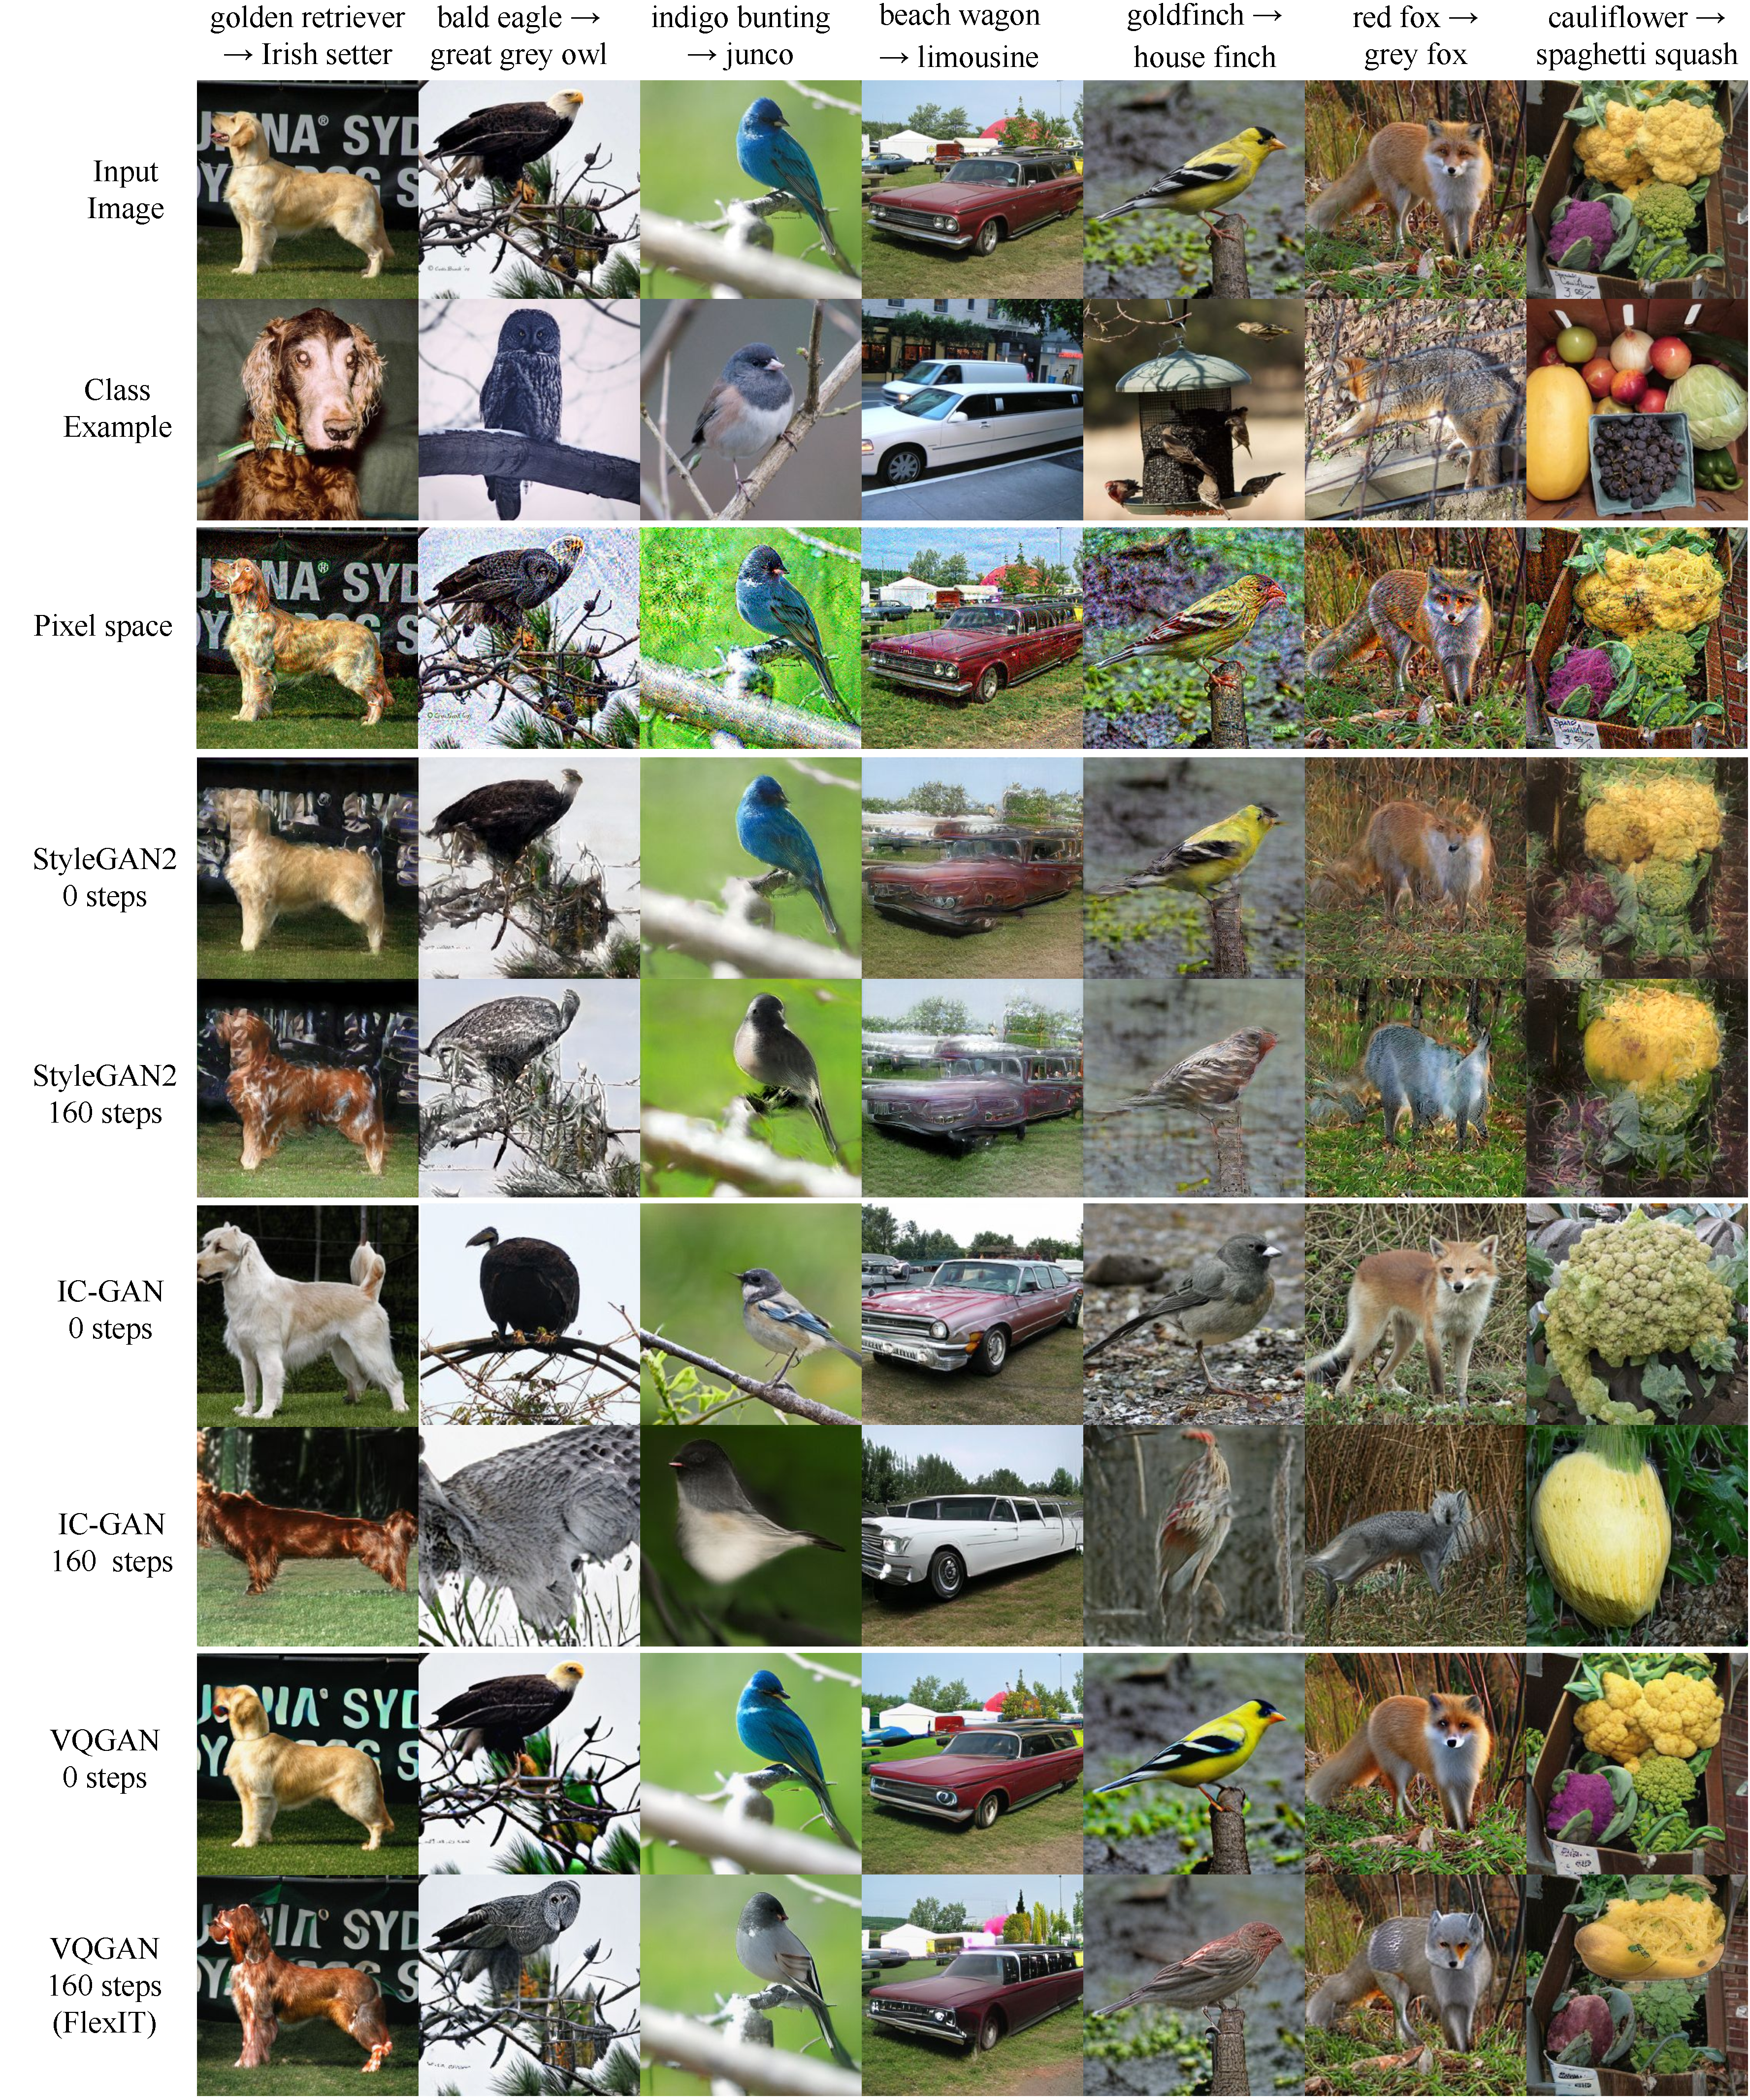
\includegraphics[width=0.85\linewidth]{images/flexit/assets/encoder2.pdf}
    \caption{
    Transformation examples with various backbones for the image latent space. For each latent space, we show the initial image decoded from the initial point $z_0$, and the resulting image after 160 optimization steps. 
    The three latent spaces differ substantially in their encoding images (0 steps). The IC-GAN latent space provides natural images that are far away from the input image due to the limited generator capacity in conjunction with the smaller latent space size (2560 dim.). StyleGAN2 images preserve the input image appearance thanks to the larger size of its latent space $\mathcal{W+}$ (8192), however images contain many unnatural artifacts due to the challenges of embedding images in this latent space \cite{tov2021designing}. The VQ-GAN latent space leads to the best  reconstruction results.
    After 160 steps of optimization, the images generated with StyleGAN2 still have the same unnatural artifacts, and images generated with IC-GAN remain natural but  far from the input images.
     %but also contain many unnatural artifacts due to its limited capacity for such diverse generation. IC-GAN images are a bit more natural but much farther away from input images due to the smaller latent space size  
    VQGAN, which we use in FlexIT, achieves good edits while preserving the overall image appearance.
    The pixel-space method introduces high-frequency artifacts, without substantially modifying the high-level semantic image content, resembling adversarial examples for image classification. 
    }
    \label{fig:encoders2}
\end{figure*}


\section{Hyperparameter study\label{hparam}}

\begin{figure}
    \centering
    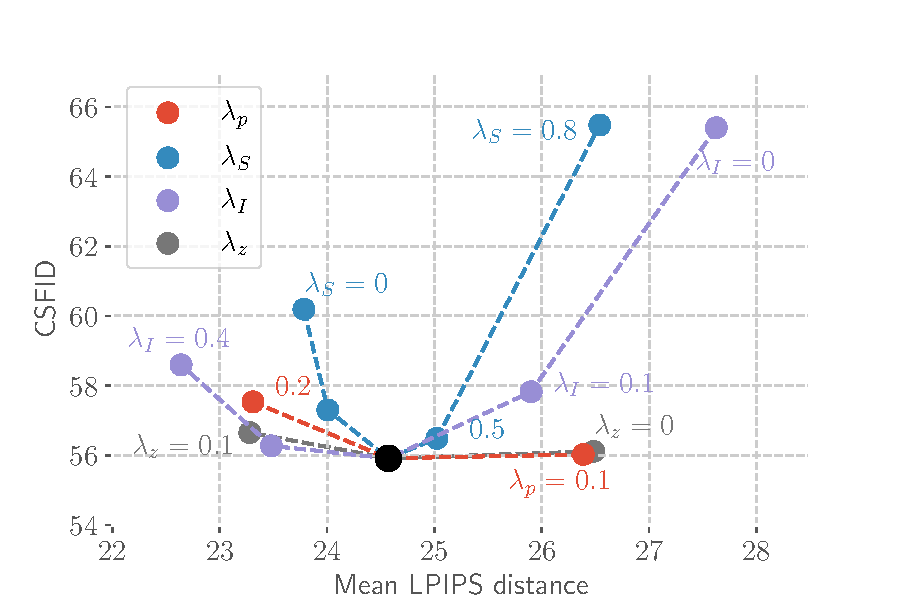
\includegraphics[width=\linewidth]{images/flexit/assets/hparam_fig.pdf}
    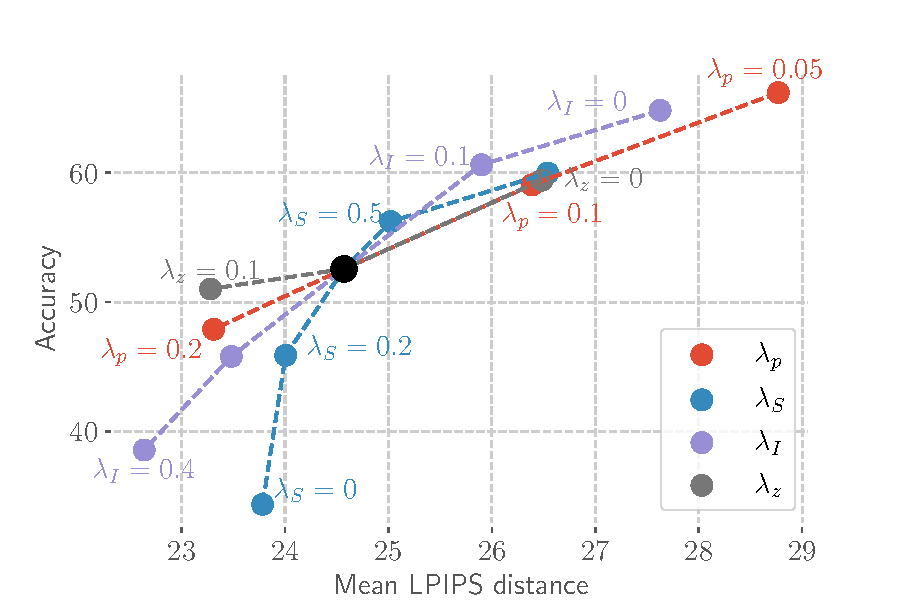
\includegraphics[width=\linewidth]{images/flexit/assets/hparam_acc.pdf}
    \caption{
    Effect  on \ac{CSFID} and Accuracy of hyper-parameters;  default settings  represented by 
    the black dot, where all lines cross.
    }
    
    \label{fig:hparam_csfid}
\end{figure}


In Figure~\ref{fig:hparam_csfid}, we illustrate the effect of our hyper-parameters on
 the \ac{LPIPS}, \ac{CSFID}, and Accuracy metrics. 
For the three regularization parameters $\lambda_p, \lambda_z, \lambda_I$, we observe
 that
(i) the \ac{LPIPS} distance with respect to the input image is smaller as the regularization 
gets stronger, as expected; 
(ii) less regularization allows more image modifications, yielding better accuracy
 scores, as illustrated in the bottom panel; 
(iii) there is a global minimum in \ac{CSFID} scores when we vary each hyper-parameter 
 independently (top panel). Regularization constraints are indeed useful to prevent
  inserting unnatural visual artifacts; however, too much regularization penalizes our 
  algorithm as the distribution of output images gets closer to the input distribution, 
  and thereby farther from the  target distribution.

The parameter $\lambda_S$, similarly to the regularization parameters, has a an optimal
 value which minimizes the \ac{CSFID}. It is beneficial to give a hint to the optimization 
 algorithm which semantic content should be changed, however focusing too much this 
 objective reduces image realism.

For our main experiments, we set our hyper-parameters to  minimize the \ac{CSFID} score on 
the development set. This is a natural choice given the convex shape of the \ac{CSFID} 
scores, whereas optimizing for accuracy  would   remove the regularizers which is 
detrimental for image quality.


\section{Limitations}

While our method  often offers compelling results, it can also fail in many cases, 
as shown in Figure~\ref{fig:failures}. While our choice of hyperparameters work well 
globally, specific images may respond poorly to the regularization parameters, as shown 
in the first three columns of Figure~\ref{fig:failures}. Our method is limited to the capacities 
of the multimodal embedding space \ac{CLIP}, which, although more semantic than the the pixel space, 
can still be prone to overfitting despite our regularizers, as shown in Figure~\ref{fig:failures} (e) 
and Figure~\ref{fig:visuresu} (last two columns). Moreover, because \ours depends on \ac{CLIP}, 
it could also inherit its biases,
such as misclassifying human faces into non-human or crime-related categories, and 
producing gender biased associations. Our editing method could reflect such biases if 
prompted transformations such as doctor $\rightarrow$ newscaster.

Our method 
works best for semantic translation when the input image provides guidance,
 but has difficulties synthesizing realistic novel objects from scratch. Other transformations 
 of interest could consider changing the 
action of a subject (person walking \vs  running), changing object attributes, 
adding or deleting objects, or consider more elaborate textual descriptions which 
require non-trivial grounding in the image (``change the color of car parked next to 
the bicycle.''). Importantly, progress in this direction will require to identify the 
right data and evaluation metrics. 


\begin{figure*}[t!]
    \center
    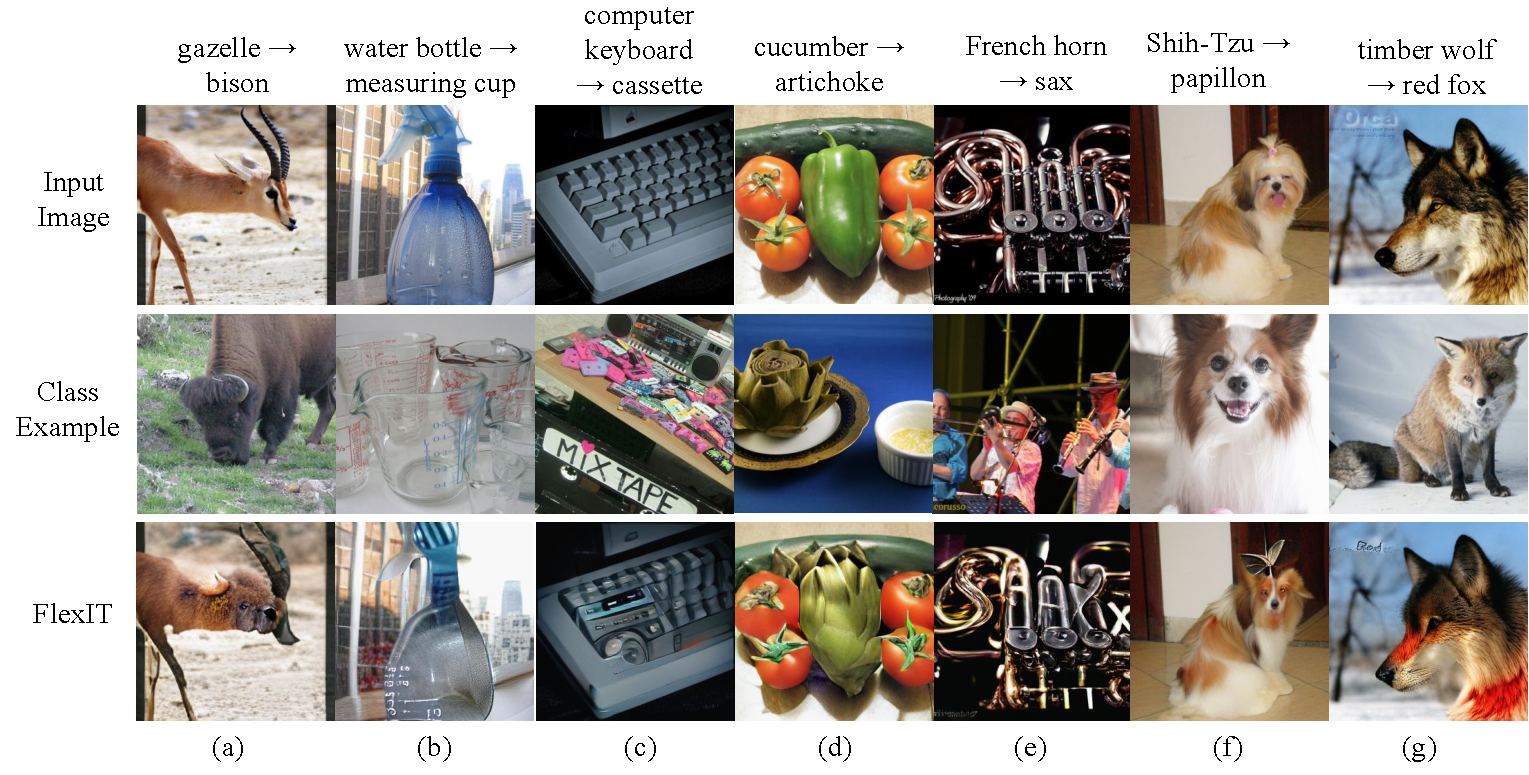
\includegraphics[width=\linewidth]{images/flexit/assets/failures.pdf}
    \caption{
    Representative failure cases of FlexIT. 
    The first three columns show examples where the regularization with respect to the initial image was too strong. (a): FlexIT added bison-like  texture but fails to change  the shape convincingly.
    (b): markings have been added to the  bottle, but without changing its  shape to that  of a measuring cup. 
    (c): only a part of the input object was changed. 
    (d): the bell pepper rather than the cucumber was transformed, probably because the former is more centered, and has a better initial shape. 
    Columns (e)--(g) show failure cases related to the \ac{CLIP} embedding space. 
    (e): we observe an interesting text synthesis behaviour where the letters of the target class ``sax'' have been written in the image. This is related to the OCR capabilities of \ac{CLIP}. 
    (f): a butterfly is synthesized on the head of the dog (\ac{CLIP} optimized for both the dog breed papillon and the insect papillon). 
    %In column 7, we see an example of undesired compositional behavior: a red fox is not actually red.
    (g): an unrealistic image is produced by adding saturated red to the image.
    }
    \label{fig:failures}
\end{figure*}

\section{Conclusion}

 We propose \ours, a novel method for semantic image translation.
 We also propose an evaluation protocol for semantic image translation, based on ImageNet,
 which we use to thoroughly evaluate our approach and its components.
 We have shown that with well-studied regularizers, we can give editing capabilities 
 to a non-generative model (the autoencoder of VQ-GAN). This allows us to circumvent the 
 problems inherent to \ac{GAN} inversion, as seen in Chapter~\ref{chapter:magec}.
 By relying on an autoencoder latent space, rather than specialized GAN latent spaces,
 it can operate on a wide range of images. Using a general pre-trained multi-modal 
 embedding space provides  flexibility, giving 
 \ours the ability to process free-text transformation queries without training.

 However, because our image generator (the decoder of VQ-GAN) is not a generative model, 
 realistic edits are not guaranteed. Later and concurrent works to this paper focus greatly 
 on Diffusion Models. In concurrent early works with editing with \ac{DDPM}s,~\cite{meng2022sdedit}, 
 for example, show that by modifying an image with strokes and then simply noising and denoising it,
 we can leverage the generative capacities of the \ac{DDPM} and turn the stroke into a realistic edit. 
 This easy inversion scheme, combined with using an actual generative prior, makes Diffusion Models 
 a perfect candidate for our work, not prone to the weaknesses of neither Chapter~\ref{chapter:magec}
 nor this chapter. In the next chapter, we will explore these models for the general task of 
 image inpainting.







